\documentclass[11pt]{amsart}
% Standard letter size paper with 1inch margins
\usepackage[letterpaper, margin=1in]{geometry}
\usepackage{algorithm, algpseudocode}
\usepackage{float}
\usepackage{amsmath, amssymb, amsthm, amsaddr}
\usepackage{enumerate, subcaption, graphicx, hyperref}
\title{AMATH 482: Homework 2}
\author{Rohan Pandey} % first and last name
\address{University of Washington, Seattle, WA
\\ \texttt{rpande@uw.edu}}
\date{\today} % you can also just type the date instead of "\today"
\begin{document}

\begin{abstract}
    This report focuses on projecting and recognizing movements of the humanoid robot OptimuS-VD, which records 38 joint movements at 60Hz. We reduce the dimensionality of the data, visualize the movements, and design an algorithm to classify actions in real-time. The dataset consists of a $114 \times 100$ matrix, representing joint positions over 1.4 seconds. Three distinct movements are recorded, and our algorithm is tested on sample data from each.
    \end{abstract}

\maketitle

\section{Introduction and Overview}\label{sec:Introduction}


In the fast-evolving world of robotics, it is essential to be able to recognize the movements of a robot in real-time. This is important for a variety of reasons, such as safety, efficiency, and even for the purpose of entertainment! In this report using Singular Value Decomposition (SVD) and Principal Component Analysis (PCA) we will project the recordings of the robot OptimuS-VD to a lower dimension and then design an algorithm that will recognize which movement OptimuS-VD is performing in real-time.

The data provided to us is a matrix of $114\times100$, where the first dimension records the locations of the joints and the second dimension the time steps. The data has been recorded for 3 different movements for 1.4 seconds and using the test sample of each movement we will test our algorithm. We also visualize the movements of the robot using the data provided to us, which will help us understand the movements of the robot better. This project is important in the field of robotics as it will help us understand the movements of the robot better and also help us recognize the movements of the robot in real-time.

In the following sections, we present the theoretical background for SVD, PCA and the Frobenius norm that was used in finding out the energy added by the singular values from SVD. We then discuss the implementation of the algorithm and then results obtained from the algorithm. We then conclude the report with a summary of the results obtained and the conclusions drawn from the results.

\section{Theoretical Background}\label{sec:theory}

\subsection{Singular Value Decomposition (SVD)}

Singular Value Decomposition (SVD) is a factorization of a matrix $A$ into three matrices $U$, $\Sigma$, and $V^T$ such that $A = U\Sigma V^T$. Here, $U$ and $V$ are orthogonal matrices and $\Sigma$ is a diagonal matrix with the singular values of $A$ on the diagonal. The singular values are the square roots of the eigenvalues of $A^TA$ or $AA^T$. The singular values are always non-negative and are arranged in descending order. The SVD is used in a variety of applications such as data compression, image compression, and in the field of robotics to analyze the movements of robots.

\subsection{Principal Component Analysis (PCA)}

PCA is a technique for reducing the dimensionality of a dataset while preserving as much variance as possible. It finds a new orthogonal basis such that:

\begin{itemize}
    \item The first principal component captures the maximum variance
    \item Each subsequent component captures the maximum remaining variance under the constraint that it is orthogonal to the previous components
\end{itemize}

Given a dataset $\mathbb{X}$ of size $m \times n$, where $m$ is the number of samples and $n$ is the number of features, PCA follows the following steps:

\begin{enumerate}
    \item Find the mean and subtract it from each feature: \[X_{\text{centered}} = X - \mu\]
    \item Compute the covariance matrix of the dataset:
    \[\Sigma = C = \frac{1}{m}X^T_{\text{centered}}X_{\text{centered}}\]
    \item Compute the SVD of the covariance matrix: \[C = U\Sigma V^T\]
    \item The principal components are the columns of $U$:
    \[Z = X_{\text{centered}}U\]
    \item Now we finally work on dimension reduction by selecting the first $k$ columns of $Z$ to get the reduced dataset $Z_k$: \[Z_k = X_{\text{centered}}U_k\] where $U_k$ is the matrix of the first $k$ columns of $U$
\end{enumerate}

PCA is a powerful technique for reducing dimensionality while preserving structure. It finds a new basis that maximizes variance and transforms data into a lower-dimensional space.

\subsection{Frobenius Norm}


The singular values from the SVD of a matrix $A$ can be used to calculate the energy of the matrix. The energy of a matrix is defined as the sum of the squares of the singular values of the covariance matrix. The Frobenius norm of a matrix $A$ is defined as \cite{wiki_frob}:

\[\|A\|_F = \sqrt{\sum_{i=1}^{r}\sigma_i^2}\]

Where $\sigma_i$ are the singular values of the matrix $A$. The Frobenius norm is used to calculate the energy of the matrix and is used in the context of PCA to find the energy added by the singular values. In terms of the modes that we are using we can determine how much variance there is from the real dataset and our prediction with this formula:

\[E_m = \frac{\sum_{i = 1}^{m} \sigma_i^2}{\sum_{i = 1}^{N} \sigma_i^2}\]

Once we get our energy we can determine how many modes we need to keep getting a good approximation of the dataset. Through SVD we can reduce the dimensionality of the dataset and still get a good approximation of the dataset by removing uncertain modes.

\section{Algorithm Implementation and Development}\label{sec:Algorithm}

The code that was needed for this report involved several key steps, using Python libraries such as \texttt{Matplotlib} \cite{matplotlib}, \texttt{NumPy} \cite{numpy}, and \texttt{Plotly} \cite{plotly}. The following algorithm outlines a general overview of the steps taken to analyze the data and project it to a lower dimension and solves all the tasks:

\begin{algorithm}
    \caption{Motion Recognition via PCA}
    \begin{algorithmic}[1]
    \State \textbf{Input:} Training samples $X_{\text{train}}$, Test samples $X_{\text{test}}$
    \State \textbf{Output:} PCA projections, classification accuracies
    \medskip
    \State \textbf{Preprocessing:}
        \State \quad Load and concatenate all training samples.
        \State \quad Center the data by subtracting the mean.
    \medskip
    \State \textbf{PCA Computation:}
        \State \quad Perform SVD on the centered data: $[U, \Sigma, V^T] \gets \text{SVD}(X_{\text{train}})$.
        \State \quad Compute and plot cumulative energy to select the number of modes.
        \State \quad Energy per mode found using Frobenius norm as: \[E_{\text{cumulative, k}} = \sum_{i = 1}^{k} \frac{s_i^2}{\sum_{j} s_j^2}\]
        where $k$ is the number of modes and $s_l$ is the $l$-th singular value.
    \medskip
    \State \textbf{Visualization:}
        \State \quad Project data onto the first 2 and 3 PCA modes.
        \State \quad Visualize trajectories in 2D and 3D spaces.
    \medskip
    \State \textbf{Classification:}
        \State \quad For each $k$ (number of PCA modes) from PCA Computation:
            \State \quad \quad Compute centroids for each movement class.
            \State \quad \quad Classify samples by assigning the label of the nearest centroid.
            \State \quad \quad Evaluate accuracy using ground truth labels.
    \medskip
    \State \textbf{Testing:}
        \State \quad Project test samples onto the PCA space.
        \State \quad Classify and evaluate performance on test data.
    \end{algorithmic}
    \end{algorithm}

\section{Computational Results}\label{sec:Results}

First let's determine using our training data, at what PCA mode do we achieve a certain amount of cumulative energy. For this task we will be testing $70\%, 80\%, 90\%, 95\%, 99\%$ cumulative energy.

Here's the results in a table:

\begin{table}[h]
    \centering
    \begin{tabular}{|c|c|}
    \hline
    \textbf{Cumulative Energy} & \textbf{Number of PCA Modes} \\ \hline
    70\%                       & 2                            \\ \hline
    80\%                       & 3                            \\ \hline
    90\%                       & 5                            \\ \hline
    95\%                       & 7                           \\ \hline
    \end{tabular}
\end{table}

The corresponding plot is below:

\begin{figure}[H]
    \centering
    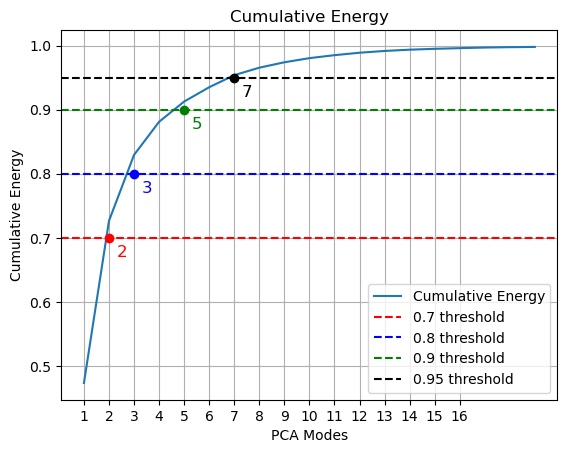
\includegraphics[width=0.6\textwidth]{PCA_mode_energy.png}
    \caption{The PCA Mode needed to achieve a certain amount of cumulative energy}
\end{figure}


Following up from the results above, we can now visualize the trajectories of the robot in 2D and 3D space (provided in the code). The following figure however only shows the 3D PCA representation of the robot's movements and includes the calculated centroids.


\begin{figure}[H]
    \centering
    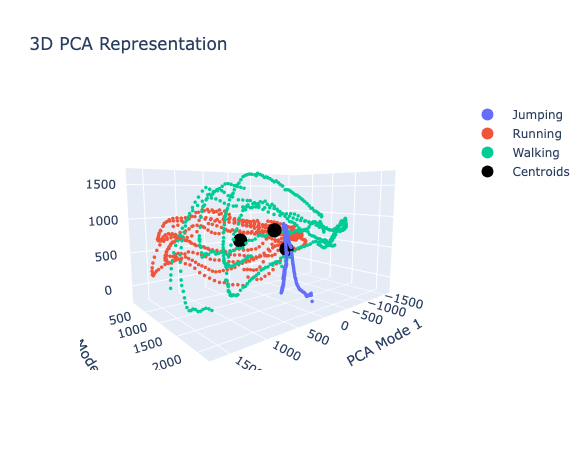
\includegraphics[width=0.8\textwidth]{3D PCA Centroid.png}
    \caption{3D Representation}
\end{figure}

Continuing on from the results above, we can work on testing the accuracy of our algorithm on the test data. The following graph shows the accuracy of the algorithm on the test data for different PCA modes, something important to notice is that the accuracy actually seems to hit an upper limit of $91.06\%$ around $k = 13$ modes.

\begin{figure}[H]
    \centering
    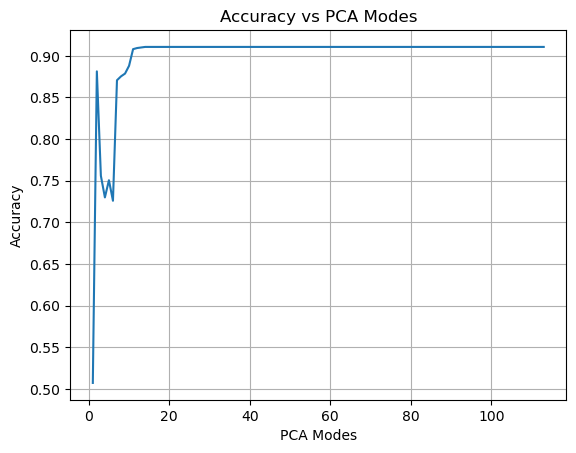
\includegraphics[width=0.4\textwidth]{train_acc.png}
    \caption{Accuracy of the algorithm on the test data}
\end{figure}

As per our tasks, we now continue on to test the algorithm on the test data and see how well it performs. And to get more accurate data we also find the accuracy of the modes that allowed us to achieve $70\%, 80\%, 90\%, 95\%, 99\%$ cumulative energy. Additionally, note that here, our constant limit seems to be around $0.9534$ for the accuracy of the algorithm on the test data.

\begin{figure}[H]
    \centering
    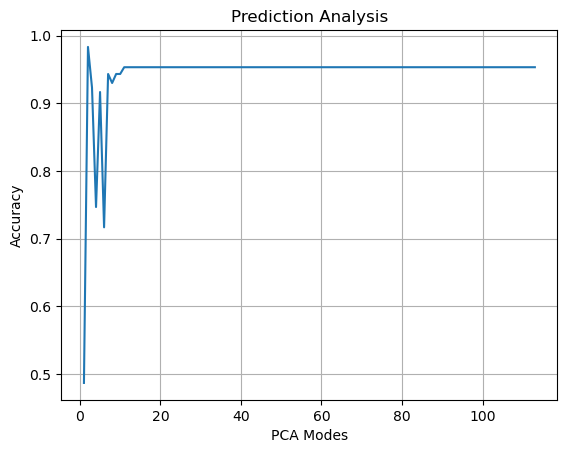
\includegraphics[width=0.4\textwidth]{test_acc.png}
    \caption{Accuracy of the algorithm on the test data}
\end{figure}



\begin{table}[H]
    \centering
    \begin{tabular}{|c|c|}
    \hline
    \textbf{Cumulative Energy} & \textbf{Accuracy} \\ \hline
    70\%                       & 0.9834                            \\ \hline
    80\%                       & 0.9234                            \\ \hline
    90\%                       & 0.9167                            \\ \hline
    95\%                       & 0.9434                           \\ \hline
    \end{tabular}
\end{table}

\section{Summary and Conclusions}\label{sec:Conclusions}


In this report, we projected the movements of the humanoid robot OptimuS-VD to a lower dimension using PCA and SVD. We visualized the movements of the robot in 2D and 3D space and designed an algorithm to classify the movements in real-time. We found that we needed 2 PCA modes to achieve $70\%$ cumulative energy, 3 modes for $80\%$, 5 modes for $90\%$, and 7 modes for $95\%$ cumulative energy. Furthermore, we also found that the accuracy of the algorithm on the training data was constant at $91.06\%$ for more than $13$ PCA modes. We also found that the accuracy of the algorithm on the test data was $98.34\%$ for $70\%$ cumulative energy, $92.34\%$ for $80\%$, $91.67\%$ for $90\%$, and $94.34\%$ for $95\%$ cumulative energy. And similarly as $k \to \infty$ the accuracy went to $0.9534$. It is interesting to compare between the train and test accuracies and see that the test accuracy is higher than the train accuracy. This might be because the test data is more structured and the algorithm is able to classify the movements better. Regardless, the algorithm shows that the training data was able to classify the movements with a relatively high accuracy, and when tested on the testing data, a similarly high performance was found. This algorithm can be used in real-time applications to classify the movements of the robot and can be used in a variety of applications such as safety, efficiency, and entertainment.


\section*{Acknowledgements}

The author is thankful to Professor Frank for providing the materials and resources needed to complete this assignment. The author is also thankful to the peers Eric Ye and Chenab for discussion and implementation of visualization techniques in Python.

\bibliographystyle{abbrv}
\bibliography{HW2_references}

\end{document}